\documentclass[a4paper, 11pt]{article}
\usepackage{comment}
\usepackage{lipsum} 
\usepackage{fullpage} %cambiar margen
\usepackage[a4paper, total={7in, 10in}]{geometry}

\usepackage{amssymb,amsthm} 
\usepackage{amsmath}
\newtheorem{theorem}{Theorem}
\newtheorem{corollary}{Corollary}
\usepackage{graphicx}
\usepackage{tikz}
\usetikzlibrary{arrows}
\usepackage{verbatim}
%\usepackage[numbered]{mcode}
\usepackage{float}
\usepackage{tikz}
\usetikzlibrary{shapes,arrows}
\usetikzlibrary{arrows,calc,positioning}
\usepackage{mathpazo} %tipo de letra 
\usepackage[utf8]{inputenc} %codificación
\usepackage[T1]{fontenc} %digitación de tildes y ñ
\usepackage[spanish]{babel} %paquete de soporte español

\tikzset{
	block/.style = {draw, rectangle,
		minimum height=1cm,
		minimum width=1.5cm},
	input/.style = {coordinate,node distance=1cm},
	output/.style = {coordinate,node distance=4cm},
	arrow/.style={draw, -latex,node distance=2cm},
	pinstyle/.style = {pin edge={latex-, black,node distance=2cm}},
	sum/.style = {draw, circle, node distance=1cm},
}
\usepackage{xcolor}
\usepackage{mdframed}
\usepackage[shortlabels]{enumitem}
\usepackage{indentfirst}
\usepackage{hyperref}

\usepackage{listings}
\lstset{literate=
  {á}{{\'a}}1
  {é}{{\'e}}1
  {í}{{\'i}}1
  {ó}{{\'o}}1
  {ú}{{\'u}}1
  {Á}{{\'A}}1
  {É}{{\'E}}1
  {Í}{{\'I}}1
  {Ó}{{\'O}}1
  {Ú}{{\'U}}1
  {ñ}{{\~n}}1
  {ü}{{\"u}}1
  {Ü}{{\"U}}1
}

\lstdefinestyle{customc}{
  belowcaptionskip=1\baselineskip,
  breaklines=true,
  frame=L,
  xleftmargin=\parindent,
  language=Python,
  showstringspaces=false,
  basicstyle=\footnotesize\ttfamily,
  keywordstyle=\bfseries\color{green!40!black},
  commentstyle=\itshape\color{purple!40!black},
  identifierstyle=\color{blue},
  stringstyle=\color{orange},
}

\lstdefinestyle{customasm}{
  belowcaptionskip=1\baselineskip,
  frame=L,
  xleftmargin=\parindent,
  language=[x86masm]Assembler,
  basicstyle=\footnotesize\ttfamily,
  commentstyle=\itshape\color{purple!40!black},
}

\lstset{escapechar=@,style=customc}



\renewcommand{\thesubsection}{\thesection.\alph{subsection}}

\newenvironment{problem}[2][Ejercicio]
{ \begin{mdframed}[backgroundcolor= red!50] \textbf{#1 #2} \\}
	{  \end{mdframed}}

% Define solution environment
\newenvironment{solution}
{\textcolor{blue}{\textbf{\textit{Solución:\\\noindent}}}}


\renewcommand{\qed}{\quad\qedsymbol}

% \\	
\begin{document}
	\noindent
	%%%%%%%%%%%%%%%%%%%%%%%%%%%%%%%%%%%%
	
	\begin{minipage}[b][1.2cm][t]{0.8\textwidth}
		\large\textbf{César Isaí García Cornejo} \hfill \textbf{Tarea 7}  \\
		cesar.cornejo@cimat.mx \hfill \\
		\normalsize Computo Científico \hfill Semestre 3\\
	\end{minipage}
	
	\hspace{14.4cm}
	\begin{minipage}[b][0.03cm][t]{0.12\linewidth}
		
		\vspace{-2.2cm}
		%%%La Ruta dependerá de donde este alojado el main y la imagen
		
\includegraphics[scale=0.3]{Figures/EscudoCimat.png}
	\end{minipage}
	
	\noindent\rule{7in}{2.8pt}
	
	%%%%%%%%%%%%%%%%%%%%%
	%%%%%%%%%%%%%%%%%%%%%%%%%%%%%%%%%%%%%%%%%%%%%%%%%%%%%%%%%%%%%%%%%%%%%%%%%%%%%%%%%%%%%%%%%%%%%%%%%%%%%%%%%%%%%%%%%%%
	% Problem 1
	%%%%%%%%%%%%%%%%%%%%%%%%%%%%%%%%%%%%%%%%%%%%%%%%%%%%%%%%%%%%%%%%%%%%%%%%%%%%%%%%%%%%%%%%%%%%%%%%%%%%%%%%%%%%%%%%%%%%%%%%%%%%%%%%%%%%%%%%
	\setlength{\parskip}{\medskipamount}
	\setlength{\parindent}{0pt}
%/////////// Ejercicio 1 /////////////////
\textbf{Con el algoritmo de Metropolis-Hastings (MH), simular lo siguiente:}
\begin{problem}{1} 
  Sean $x_i \sim Ga(\alpha,\beta)$ $i =1,2,\cdots,n$. Simular datos $x_i$ con $\alpha = 3$ y $\beta = 100$ considerando los casos $n=4$ y 30.
  
  Con $\alpha \sim U(1,4)$, $\beta \sim exp(1)$ distribuciones a priori, se tiene la posterior 
  \begin{align*}
    f(\alpha, \beta|\bar{x} ) \propto \frac{\beta^{n\alpha}}{\Gamma(\alpha)}^{n }  r_1^{\alpha-1}e^{-\beta(r_2 + 1)} \mathbb{1}_{1 \leq \alpha \leq 4} \mathbb{1}_{b>1}
  \end{align*}
  con $r_2 = \sum_{i=1}^{n } x_i$ y $r_1 = \prod_{i =1}^{n }x_i$.
  En ambos casos, grafica los contornos para visualizar dónde está concentrada la posterior.
  Utilizar la propuesta
  \begin{align*}
    q \left(\binom{\alpha_p }{\beta_p }| \binom{\alpha}{\beta}\right) = \binom{\alpha}{\beta} + \binom{\varepsilon_1}{\varepsilon_2}
  \end{align*}
  donde
  \begin{align*}
    \binom{\varepsilon_1}{\varepsilon_2} \sim N \left(\binom{0}{0}, \begin{pmatrix}
      \sigma_1^2 &0 \\ 
      0 & \sigma_2^2 
      \end{pmatrix} \right)
  \end{align*}

\end{problem}

\begin{solution} 
  Se implementa el algoritmo de Metropolis- Hastings con caminatas aleatorias para la posterior mostrada en el enunciado para cada caso, es decir, $n=4$ y $n = 30$

  Se procede definiendo una función que calcule la distribución posterior según ciertos valores de $\alpha,\beta$. Como es una función bivariada, y con objetivo de visualizar la distribución posterior, es que se grafican las curvas de nivel. Notemos que el soporte está en $1 \leq \alpha \leq 4$ y $\beta > 0$. Tenemos las siguientes gráficas
  \begin{figure}[H] 
      \centering 
      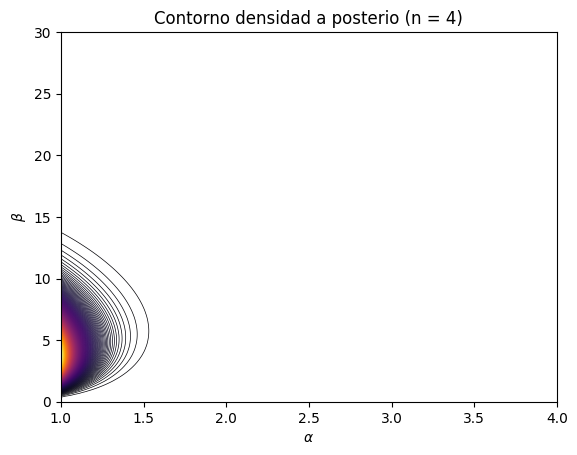
\includegraphics[width = 12 cm ]{Figures/contorno1.png} 
      \caption{Grafica de contornos para $n = 4$}
      \label{Fig. 1.01}
  \end{figure} 
  \begin{figure}[H] 
      \centering 
      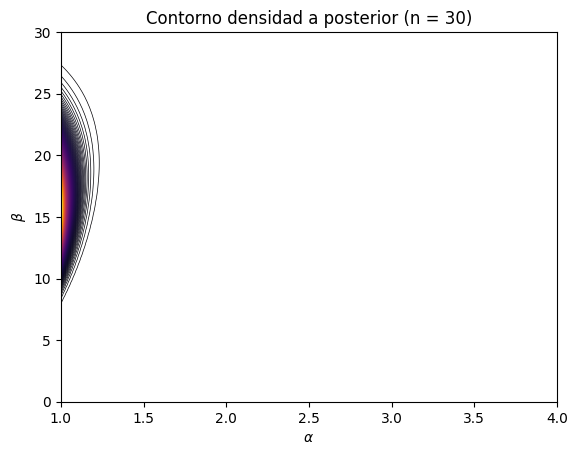
\includegraphics[width = 12 cm ]{Figures/contorno2.png} 
      \caption{Grafica de contornos para $n = 30$}
      \label{Fig. 1.02}
  \end{figure} 
  Notemos que tenemos una concentración para $\alpha $ pegados al extremos izquierdo del soporte, mientras que para $\beta$ se aglomeran por 5 o 15 dependiendo de $n$.

  Aplicando el método de Metropolis-Hastings con caminata aleatoria y punto inicial en $\alpha = 3,\beta = 40$ y propuesta como es indicada en el enunciado
  \begin{align*}
    \varepsilon_1 \sim N(0, \sigma_1^2) \:\:\:\:\:\: \varepsilon_2 \sim N(0,\sigma_2^2)
  \end{align*}
  con $\sigma_1 =$ 0.05 y $\sigma_2^2$ = 0.5
  
  Como la propuesta es simétrica 


















\end{solution}

\begin{problem}{2} 
  Simular de la distribución Gamma($\alpha$,1) con la propuesta Gamma($[\alpha], 1 $), donde $[a]$ denota la parte entera de $[a]$.

  Además, realizar el siguiente experimento: poner como punto inicial $x_0 = 900$ y graficar la evolución de la cadena, es decir, $f(X_t)$ vs $t$.
\end{problem}

\begin{solution} 
  
\end{solution}

\begin{problem}{3} 
  Implementar Random Walk Metropolis Hasting (RWMH) donde la distribución objetivo es $\mathcal{N}_2 \left( \mu, \Sigma  \right)$, con 
  \begin{align*}
    \mu = \binom{3}{5} \:\:\:\:\: \Sigma = \begin{pmatrix}
      1 & 0.9 \\ 
      0.9 & 1 
      \end{pmatrix}.
  \end{align*}
  Utilizar como propuesta $\varepsilon_i \sim \mathcal{N}_2(0,\sigma^2I)$ ?` Cómo elegir $\sigma$ para que la cadena sea eficiente ? ?` Qué consecuencias tiene la elección de $\sigma$ ?

  Como experimento, elige como punto inicial $x_0 = \binom{1000}{1}$ y comenta los resultados.
\end{problem}

\textbf{Para todos los incisos del ejercicio anterior:}
\begin{enumerate}
  \item Establece cual es tu distribución inicial .
  \item Grafica la evolución de la cadena.
  \item Indica cuál es el Burn-in.
  \item Comenta qué tan eficiente es la cadena.
  \item Implementa el algoritmo MH considerando una propuesta diferente.
\end{enumerate}

\begin{solution} 
  
\end{solution}

\begin{thebibliography}{9}

    \bibitem{Casella}
    Robert, C. P., Casella, G., and Casella, G. (1999). Monte Carlo statistical methods (Vol. 2). New York: Springer.

    \bibitem{Wasserman}
    Wasserman, L. (2004). All of statistics: a concise course in statistical inference (p. 413). New York: Springer.
    
\end{thebibliography}
      




    \end{document}